% !TEX encoding = UTF-8
% !TEX program = xelatex
\documentclass[12pt,a4paper]{article}
\usepackage[paperwidth=210mm, paperheight=297mm, left=0.75in, right=0.75in, bottom=1in, top=1in]{geometry}
\usepackage{polyglossia}
\setdefaultlanguage[babelshorthands]{italian}
\usepackage{fontspec}
\usepackage{graphicx}
\usepackage{blindtext}
\usepackage{wrapfig}

\frenchspacing
\makeindex

\begin{document}
\title{\vspace{-70pt}Hubble}
\author{Paolo Vincenzi}
\date{}
\maketitle
\pagestyle{empty}
\thispagestyle{empty}

\section*{Storia}
\label{storia}
\begin{wrapfigure}{r}{0.35\textwidth}
  \vspace{-10pt}
  \begin{center}
    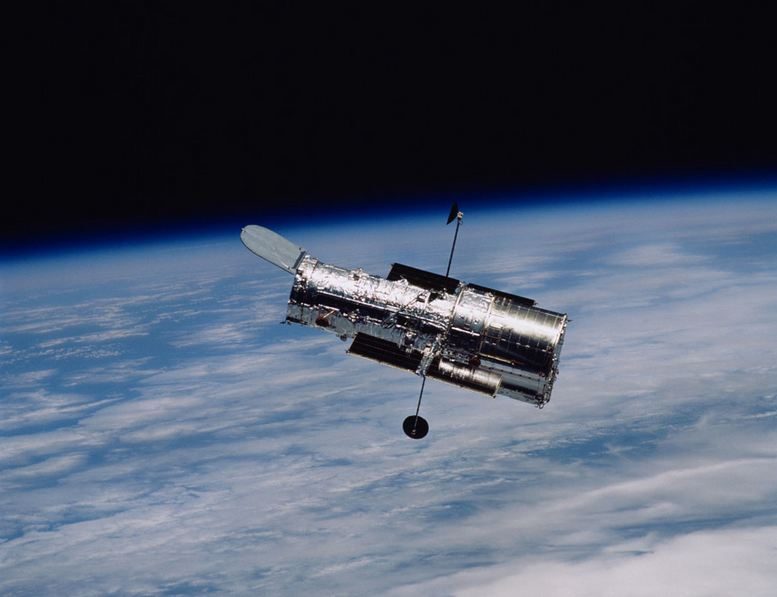
\includegraphics[width=0.30\textwidth]{satellite}
  \end{center}
  \vspace{-20pt}
\end{wrapfigure}
L'Hubble Space Telescope è un programma cooperativo dell'ESA (European Space Agency) e della NASA (National Aeronautics and Space Administration) per la gestione dell'\emph{osservatorio spaziale} a lunga durata, a beneficio della comunità astronomica internazionale. L'HST è un osservatorio concepito per la prima volta nel 1940, progettato e costruito tra il 1970 e il 1980 e divenuto finalmente operativo solo nel \emph{1990}. Fin dal suo inizio, l'HST fu progettato come un tipo molto particolare di missione per la NASA: il fatto di essere un osservatorio permanente implica la pianificazione di regolari missioni di servizio per riparare guasti e sostituire apparecchiature superate dal progresso tecnologico.
Per lo studio completo di un oggetto celeste, è necessario traportare gli strumenti di misura al di sopra dell'atmosfera mediante palloni sonda o razzi.
Il telescopio spaziale, dato che opera al di fuori dell'atmosfera, consente un incremento nella magnitudine limite, ma soprattutto una visione ``a tutto spettro'' della volta celeste.

\section*{Osservazioni}
\label{osservazioni}

Il telescopio ha una massa di circa 11 tonnellate, è lungo 13,2 metri, ha un diametro massimo di 2,4 metri ed è costato 2 miliardi di dollari. Si tratta di un riflettore con due specchi in configurazione Ritchey-Chrétien. Lo specchio primario è uno specchio iperbolico concavo di 2,4 metri di diametro, che rinvia la luce su uno specchio iperbolico convesso di circa 30 centimetri di diametro. La distanza fra i vertici dei due specchi è di 4,9 metri. Approssimando i due specchi come sferici, si può calcolare il punto di formazione del fuoco Cassegrain, ottenendo che l'immagine si forma circa 1,5 metri dietro il primario.
Due pannelli solari generano l'elettricità, che serve principalmente per alimentare le fotocamere e i tre giroscopi usati per orientare e stabilizzare il telescopio. In 20 anni di carriera Hubble ha ripreso più di 700.000 immagini astronomiche.
A bordo dell' HST troviamo una camera planetaria grandangolare, un spettrografo(STIS), una camera a infrarossi e spettrometro multi-oggetto(NICMOS), una camera per oggetti deboli(FOC) e delle ottiche correttive assiali(COSTAR).

Il telescopio spaziale Hubble fino ad ora ha compiute numerose scoperte:

\begin{itemize}
\item Riprese eccezionali immagini della collisione della cometa Shoemaker-Levy 9 con il pianeta Giove nel 1994.

\item Fu il primo telescopio a raccogliere delle prove del fatto che dei pianeti siano presenti anche attorno a stelle diverse dal Sole

\item Ha dimostrato che la materia oscura della nostra galassia non può essere formata solo da deboli stelle non ancora osservate

\item Effettuò numerose osservazioni a una parziale conferma della teoria che la maggior parte delle galassie contengono un buco nero nel loro nucleo

\item Nel dicembre 1995, Hubble riprese un'immagine chiamata lo Hubble Deep Field, una regione grande un trentesimo di milionesimo del cielo notturno e contenente numerose migliaia di deboli galassie, rafforzando l'ipotesi che l'Universo sia uniforme su vasta scala, e che la Terra occupi un posto come gli altri nell'Universo.

\item Nel 2010, è stata scoperta la galassia più lontana da noi, circa 13,2 miliardi di anni luce, il che equivale a un'osservazione di quello che era l'universo 480 milioni di anni dopo il Big Bang.

\item Il 20 luglio 2011 è stato scoperto il quarto satellite di Plutone.

\item L'11 luglio 2012 è stato scoperto un altro satellite di Plutone, il quinto.

\end{itemize}


\end{document}